\documentclass[a4paper, 12pt, one column, aas_macros]{article}

\usepackage[italian]{babel}
\usepackage[utf8x]{inputenc}
\usepackage[T1]{fontenc}

\usepackage[top=1.3cm, bottom=2.0cm, outer=2.5cm, inner=2.5cm, heightrounded,
marginparwidth=1.5cm, marginparsep=0.4cm, margin=1.5cm]{geometry}

\usepackage{graphicx}
\usepackage[colorlinks=False]{hyperref} 
\usepackage{amsmath}  
\usepackage{amsfonts} 
\usepackage{amssymb}  

\usepackage[authoryear]{natbib}
\bibliographystyle{abbrvnat}
\setcitestyle{authoryear,open={(},close={)}}

\usepackage{pdfpages}
\usepackage{graphicx}
\usepackage{subfigure}
\usepackage{array}
\usepackage{siunitx}
\usepackage{booktabs}
\usepackage[italiano]{algorithm2e}
\SetKwComment{Comment}{/* }{ */}

\DeclareSIUnit[]{\byte}{B}
\DeclareSIUnit[]{\bit}{bit}

\title{iCipher, un'applicazione in C++ per cifrare frasi e parole con delle rivisitazioni degli algoritmi più famosi}
\author{Lorenzo LEONI}
\date{%
	Università degli studi di Bergamo, Dipartimento di Ingegneria Gestionale, dell'Informazione e della Produzione\\[2ex]%
	\today
}

\begin{document}
	\maketitle
	
	\section{Introduzione}
	Esiste un modo per complicare e per rendere meno vulnerabili alcuni degli algoritmi di cifratura a sostituzione monoalfabetica più rinomati quali Cesare e Vigenère? L'obiettivo di iCipher è proprio questo, ovvero fornire all'utente un'applicazione in C++ attraverso la quale possa cifrare e decifrare frasi e parole utilizzando degli algoritmi più complessi, derivanti da quelli sopracitati.
	
	\section{Funzionalità}
	Attraverso un'interfaccia a riga di comando, l'utente ha la possibilità di accedere tramite iCipher a due servizi:
	\begin{itemize}
		\item \textbf{cifratura} e \textbf{decifrazione} di sequenze di caratteri tramite il cifrario di Cesare e la sua versione modificata, l'algoritmo di Vigenère e il cifrario di Leoni, una tecnica che itera $n$ volte le precedenti;
		\item \textbf{memorizzazione} in un file CSV delle versioni criptate delle parole che sono state inserite nel programma. Per ognuna di esse vengono specificati anche i parametri dell'algoritmo di cifratura che è stato utilizzato.
	\end{itemize}
	L'applicazione opera completamente offline, pertanto non si corre il rischio di diffondere in rete i propri dati sensibili.
	
	\section{Architettura}
	Le classi necessarie per l'implementazione delle funzionalità di iCipher sono state raggruppate in \num{3} file header:
	\begin{itemize}
		\item \textbf{encryptors.h} (figura \ref{UML_1});
		\item \textbf{application.h} e \textbf{consts.h} (figura \ref{UML_2});
	\end{itemize}
	Tutte le classi (fatta eccezione per \verb|Application|) sono state definite utilizzando il costrutto \verb|struct| piuttosto che \verb|class|; tale scelta risiede nel voler tenere meglio sotto controllo la visibilità dei campi, dei metodi e la tipologia di ereditarietà essendo \verb|public| di default con il costrutto \verb|struct|. 
	
	\begin{figure}[t!]
		\centering
		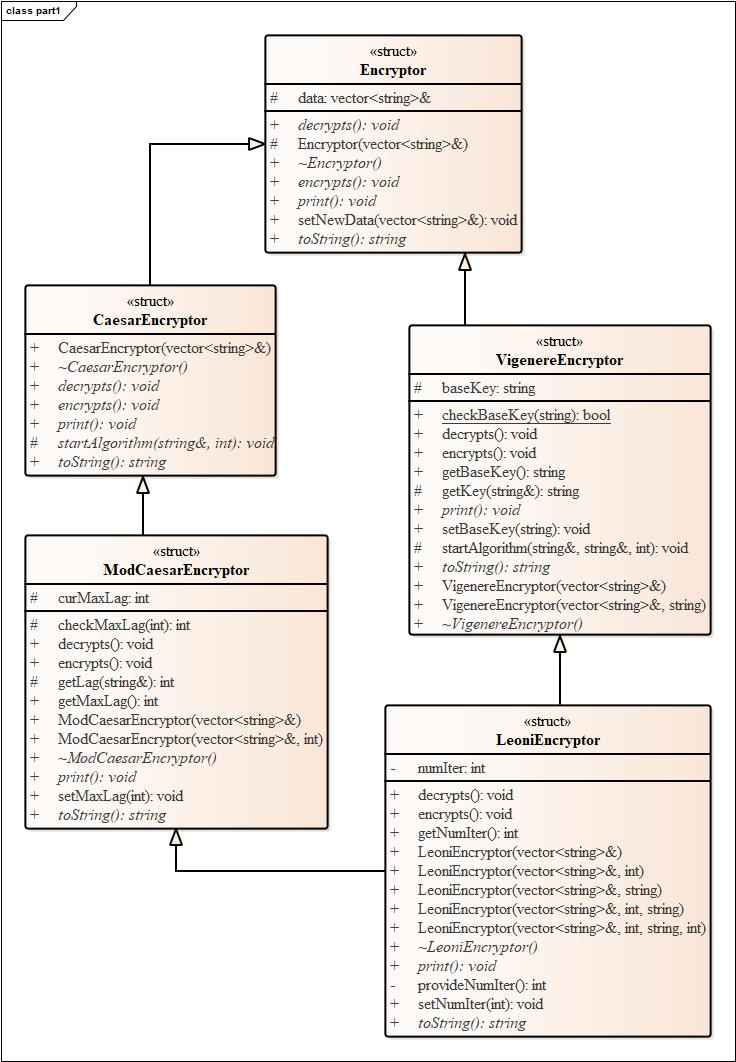
\includegraphics[height=550px]{UML/UML_1.jpg}
		\caption{diagramma UML delle classi dichiarate in \textit{encryptors.h}.}
		\label{UML_1}
	\end{figure}
	\subsection{Header encryptors}
	La gerarchia tra le classi aventi il compito di implementare gli algoritmi di cifratura è stata organizzata in modo tale da realizzare un \textit{struttura a diamante}. La \verb|struct Encryptor| definisce i prototipi delle funzioni \verb|encrypts()|, \verb|decrypts()|, \verb|toString()| e \verb|print()|; esse sono dichiarate \verb|virtual|, pertanto le classi derivate possono implementarle. Da notare che il costruttore di \verb|Encryptor| riceve come argomento il riferimento alla struttura dati di stringhe \verb|vector<string>| contenente le parole da cifrare o decifrare; ciò permette ai metodi \verb|encrypts()| e \verb|decrypts()| di agire direttamente sul vettore target, senza la necessità di creare una sua copia locale. Proseguendo nella descrizione della gerarchia, si osserva che sia \verb|CaesarEncryptor| sia \verb|VigenereEncryptor| ereditano pubblicamente e \textit{virtualmente} dalla classe base. Tale scelta è necessaria affinché \verb|LeoniEncryptor| erediti una sola volta da \verb|Encryptor| (per via dell'ereditarietà multipla), ovvero si vuole evitare che vengano a crearsi due istanze distinte di quest'ultima classe nell'istante in cui viene invocato uno dei costruttori di \verb|LeoniEncryptor|. Infine, nel diagramma UML non è specificato, però è importante sottolineare una differenza: \verb|CaesarEncryptor| e \verb|VigenereEncryptor| \textit{implementano} le interfacce dei metodi della classe \verb|Encryptor|, mentre \verb|ModCaesarEncryptor| effettua l'\textit{overriding} degli stessi poiché ne eredita le implementazioni dalla sua classe base \verb|CaesarEncryptor|.
	
	\begin{figure}[t!]
		\centering
		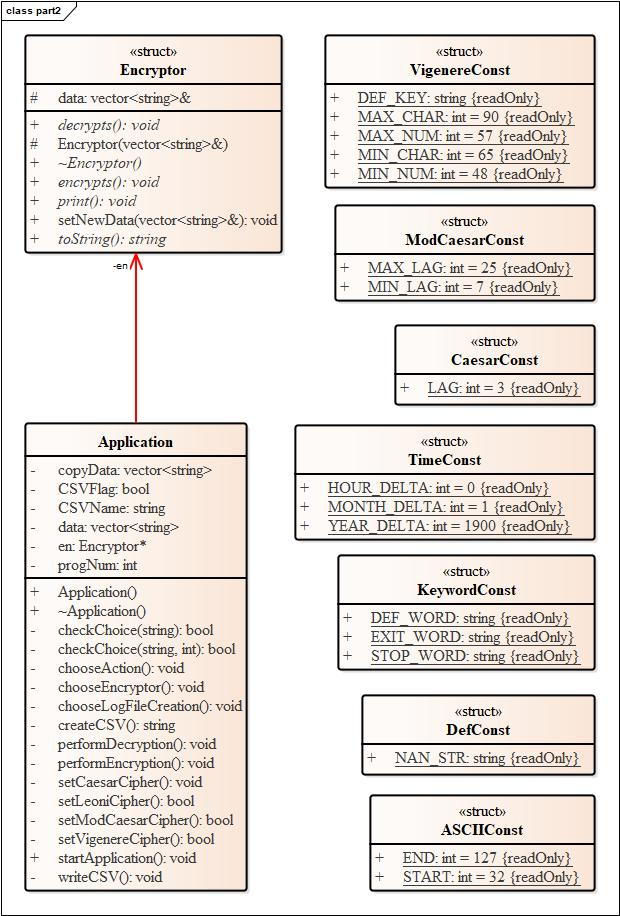
\includegraphics[height=500px]{UML/UML_2.jpg}
		\caption{diagramma UML delle classi dichiarate in \textit{application.h} e in \textit{const.h}.}
		\label{UML_2}
	\end{figure}
	\subsection{Header application e consts}
	La classe \verb|Application| è il cuore di iCipher, l'hub dal quale è possibile accedere a tutte le funzionalità dell'applicazione in C++. Il campo \verb|en| è un puntatore a un oggetto di tipo \verb|Encryptor|; grazie alla gerarchia sopracitata, è possibile assegnare alla variabile \verb|en| il riferimento a un qualsiasi oggetto che eredita, direttamente o indirettamente, da \verb|Encryptor|, istanza che cambia a seconda del cifrario che l'utente desidera utilizzare. Ciò è reso possibile dal \textit{binding dinamico} (il quale viene abilitato dichiarando \verb|virtual| i metodi di \verb|Encryptor|): il compilatore risolve l'overriding in fase di esecuzione (\textit{late binding}). Le classi definite in \textit{consts.h}, invece, servono per fissare le costanti che vengono utilizzate dall'applicazione e dagli algoritmi di cifratura, per esempio gli intervalli di caratteri della tabella ASCII che possono essere utilizzati per la cifratura e per la definizione della chiave per il cifrario di Vigenère. La decisione di creare un file header apposta per le costanti risiede nella comodità di poterle modificare all'occorrenza da un unico file, senza così andare a rintracciarle singolarmente all'interno del codice. 

	\section{Cifrario di Leoni}
	
	L'algoritmo si basa sull'utilizzo combinato e iterato dei cifrari di Cesare modificato\footnote{per una descrizione accurata dell'algoritmo si rimanda alla documentazione di PasswordCollector, sezione \num{5}: \url{https://github.com/lamferzon/PasswordCollector/blob/main/documentazione/documentazione.pdf}} e di Vigenère. Gli algoritmi \ref{alg1} e \ref{alg2} descrivono rispettivamente la cifratura e decifrazione. Si ricorda che la versione modificata dell'algoritmo di Cesare aggiunge un carattere in coda alla parola criptata in modo tale che ci sia la possibilità di risalire al $lag$ (scelto casualmente) utilizzato, quindi \textit{n} iterazioni comportano l'aggiunta di \textit{n} caratteri alla parola originale.
	\begin{algorithm}
		\caption{algoritmo di cifratura del cifrario di Leoni}\label{alg1}
		$nIter \gets$ \textit{ numero di iterazioni};\\
		$data[ \ ] \gets$ \textit{vettore di stringhe da criptare};\\
		$key \gets$ \textit{chiave crittografica per il cifrario di Vigenère}; \verb|/* es. ULIVETO11 */|\\
		$i \gets 0$;\\
		\While{$ i < length(data)$}{
			$data[i] \gets encrypts(data[i]$, \textit{“Vigenère”}, $key$);\\
			$data[i] \gets encrypts(data[i]$, \textit{“ModCaesar”});\\
			$ i = i + 1$;\\
		}
	\end{algorithm}
	\begin{algorithm}
		\caption{algoritmo di decifrazione del cifrario di Leoni}\label{alg2}
		$nIter \gets$ \textit{numero di iterazioni};\\
		$data[ \ ] \gets$ \textit{vettore di stringhe da criptare};\\
		$key \gets$ \textit{chiave crittografica per il cifrario di Vigenère};\\
		$i \gets 0$;\\
		\While{$ i < length(data)$}{
			$data[i] \gets decrypts(data[i]$, \textit{“ModCaesar”});\\
			$data[i] \gets decrypts(data[i]$, \textit{“Vigenère”}, $key$);\\
			$ i = i + 1$;\\
		}
	\end{algorithm}
	
	\section{Documento CSV}
	Se si desidera, iCipher dà la possibilità di salvare le versioni crittografate delle proprie parole o frasi all'interno di un file CSV. Per ognuna di esse vengono specificati anche i parametri dell'algoritmo che è stato utilizzato. Di seguito è riportato un esempio di documento CSV:
	\begin{verbatim}
		ProgNum,Password,EncryptorType,MaxLag,BaseKey,NumIter,(CryptedPw)
		1,Lor3nzo-1998,Caesar cipher,3,//,//,(Oru6q}r04<<;)
		2,Lor3nzo-1998,Modified Caesar cipher,25,//,//,(X{~?z&{9=EED>)
		3,Lor3nzo-1998,Vigenere cipher,//,ULIVETO11,//,(A[[)Sn^^b.%!)
		4,Lor3nzo-1998,Leoni cipher,25,ULIVETO,7,(gK9Uy.`Hm`[CBM";.JW)
	\end{verbatim}
	
	\section{Repository GitHub}
	Il codice sorgente di iCipher è disponibile per il download al seguente repository:
	\begin{center}
		\url{https://github.com/lamferzon/iCipher}
	\end{center}
	\begin{figure}[h!]
		\centering
		\subfigure[]{\label{Screen1}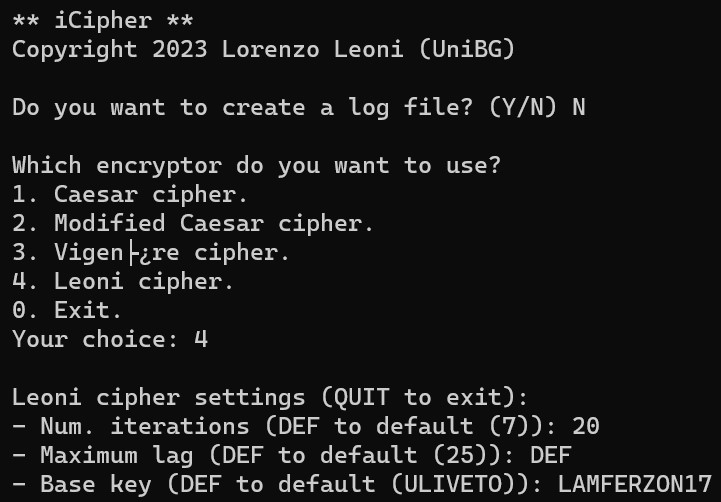
\includegraphics[height=200px]{Immagini/Screenshot1.jpg}}
		\subfigure[]{\label{Screen2}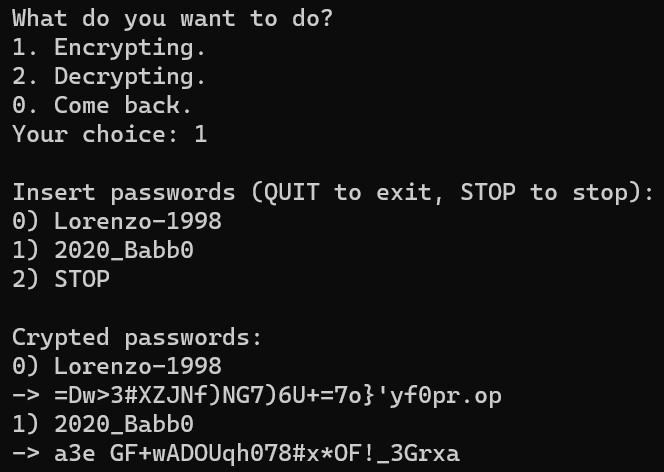
\includegraphics[height=200px]{Immagini/Screenshot2.jpg}}
		\caption[]{un paio di screenshot dell'applicazione in esecuzione.}
		\label{App_screens}
	\end{figure}
	
\end{document}